\documentclass[10pt,a4paper]{article}
\usepackage[T1]{fontenc}
\usepackage[utf8]{inputenc}
\usepackage{lmodern}
\usepackage[margin=25mm]{geometry}
\usepackage{amsmath,amssymb,booktabs,graphicx}
\usepackage{caption,float}
\usepackage[hidelinks]{hyperref}
\captionsetup{font=small}
\setlength{\parindent}{0pt}
\setlength{\parskip}{5pt}
\setlength{\emergencystretch}{2em}
\newcommand{\ind}{\mathbf{1}}
\newcommand{\Ptop}{\widehat{P}_{46}}
\begin{document}
\hypersetup{pdftitle={Point 2: Uncertainty-adjusted hazard ranking}}
\section*{Point 2: Uncertainty-adjusted hazard ranking}
\section{Evaluation setup}
We analyze hazard probabilities from $B=128$ separately fitted linear heads over
frozen DINOv3 ViT-B/16 features. Each head was trained on a bootstrap sample of
1,276 Pittsburgh training observations (527 hazards and 749 non-hazards), with
exact-pixel clusters sampled within strata defined by their binary-label composition.
All heads used Adam, learning rate $3\times10^{-5}$, weight decay $0.01$, batch
size 64, 5,000 updates, unweighted binary cross-entropy, and the final checkpoint.

The validation set contains 382 observations, including 157 hazards; the test set
contains 380 observations, including 174 hazards. The review budget is fixed at
$k=46$: 12.04\% of validation and 12.11\% of test. For an ordering $\pi$, the metrics are
\begin{equation}
\operatorname{Precision@46}=\frac{1}{46}\sum_{a=1}^{46}y_{\pi(a)},
\qquad
\operatorname{Recall@46}=\frac{\sum_{a=1}^{46}y_{\pi(a)}}{\sum_{i=1}^{N}y_i},
\end{equation}
where $y_i=1$ denotes a hazard. Subtype predictions are excluded.

\section{Uncertainty-adjusted scores}
Let $p_i^{(b)}$ be head $b$'s hazard probability for observation $i$. Define
\begin{equation}
\mu_i=\frac{1}{B}\sum_{b=1}^{B}p_i^{(b)},\qquad
s_i=\sqrt{\frac{1}{B-1}\sum_{b=1}^{B}(p_i^{(b)}-\mu_i)^2},\qquad
S_i(\lambda)=\mu_i-\lambda s_i.
\end{equation}
Images are ranked by decreasing $S_i$. Here $s_i$ is the sample standard deviation
across heads, not the standard error of their average. Scores are not clipped to
$[0,1]$; exact score ties are resolved by ascending sample ID.

We search 81 prespecified values $\lambda\in\{0,0.05,\ldots,4\}$, maximizing
validation precision@46. Ties are resolved by the smallest $\lambda$. The selected
value is frozen before test evaluation. Mean-probability ranking ($\lambda=0$)
and a fixed fifth-percentile probability score are comparators; the latter does
not participate in selection. No parameter is selected using test labels.

\section{Results}
The best validation result is 34 hazards among 46 selected images
(73.91\% precision). Eight grid values, $\lambda=0$ through $0.35$, tie for this
result. The tie rule therefore selects $\lambda=0$, so the selected method is
exactly mean-probability ranking. All remaining grid values ($0.40$--$4.00$)
retrieve 33 validation hazards (71.74\%). This is selection within the searched
grid, not a claim about every real-valued penalty.
\begin{table}[H]
\centering
\caption{Hazard retrieval at the fixed budget of 46 images. Precision and recall are percentages.}
\label{tab:adjusted}
\small
\begin{tabular}{llrrr}
\toprule
Split & Ranking & Hazards & Precision@46 & Recall@46 \\
\midrule
Validation & Mean probability & 34/46 & 73.91 & 21.66 \\
 & Selected $\mu-\lambda s$ ($\lambda=0$) & 34/46 & 73.91 & 21.66 \\
 & Fifth probability percentile & 32/46 & 69.57 & 20.38 \\
\midrule
Test & Mean probability & 27/46 & 58.70 & 15.52 \\
 & Selected $\mu-\lambda s$ ($\lambda=0$) & 27/46 & 58.70 & 15.52 \\
 & Fifth probability percentile & 26/46 & 56.52 & 14.94 \\
\bottomrule
\end{tabular}
\end{table}
\begin{figure}[htbp]
\centering
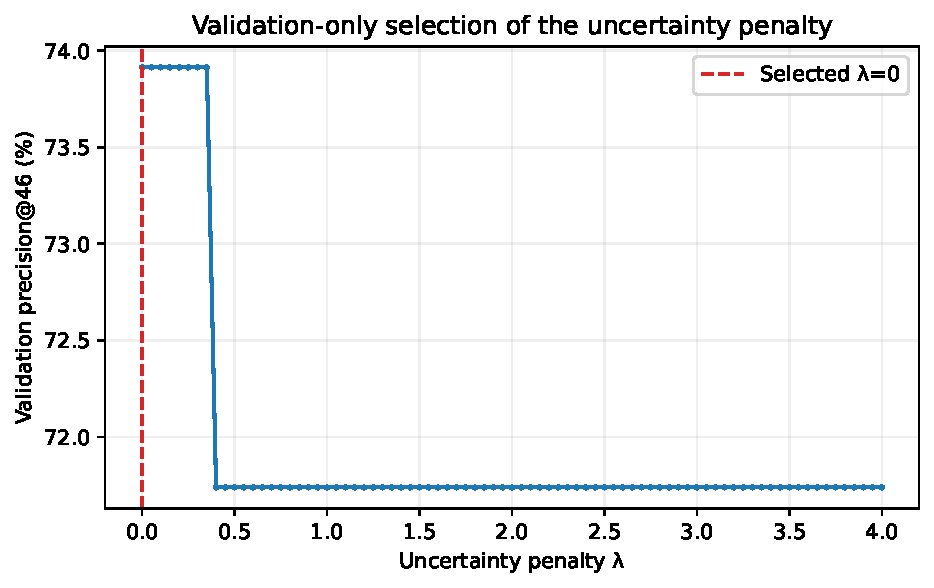
\includegraphics[width=.87\linewidth]{figures/point_2_validation_lambda_sweep.pdf}
\caption{Validation precision@46 over the uncertainty-penalty grid. The smallest maximizer, $\lambda=0$, is selected.}
\label{fig:lambda}
\end{figure}

\section{Interpretation}
The selected ranking retrieves 27 test hazards (58.70\% precision@46;
15.52\% recall@46). The fixed fifth-percentile comparator retrieves 26
(56.52\% precision; 14.94\% recall). Thus, neither conservative scoring approach
improves retrieval here: the validation-selected SD penalty is zero, and the
lower-quantile comparator performs worse on both splits.

If the mean probabilities equal the relevant predictive expectations, choosing
the largest means maximizes the expected number of hazards at a fixed review
budget. An SD penalty instead expresses a preference for stability; it need not
increase hazard yield. Each extra correct retrieval changes precision@46 by
2.17 percentage points. The validation optimum was used for selection and is
therefore optimistic; these results do not establish a population-level or
statistically significant improvement.

\section{Limitations}
The 128 heads share a frozen representation and overlapping bootstrap training
samples. Their variation measures sensitivity to these model refits, not all
sources of predictive uncertainty. Empirical intervals are not automatically
calibrated posterior intervals or confidence intervals for population precision.
Original evaluation observations are retained, including duplicate pixel groups
and groups with conflicting hazard labels: 18 duplicate groups, of which 6 have
conflicting labels, in validation; 12 and 2, respectively, in test. Shared confident
mistakes and label conflicts can therefore persist across the ensemble.

\end{document}
